\documentclass{article}

\usepackage[a4paper, total={6in, 8in}]{geometry}
\usepackage{graphicx}
\usepackage{subfiles}




\begin{document}

\section{Introduction}

\noindent This Project is a proposal from the professor Christian Langen from the Hochschule Karlsruhe with the intention of being a learning experience for the students. There are probably better methods, software and hardware to develop the project, neverthless this is the final product we could do with the given Software, Hardware and Knowledge. 

\section{Development}

\subsection{Main Idea}

\noindent The aim of the project is to make an instrument, that can be played without making any physical contact with it. To this purpose we count with three hardware components, an E-field sensor (MGC3031), a microcontroller (STM32F4 - Discovery Board) and a Computer with Matlab/Simulink installed. The project can be divided into 3 main tasks, communicating with the sensor, processing the sensor's data and outputing the sound.  

\begin{figure}[h]
\centering
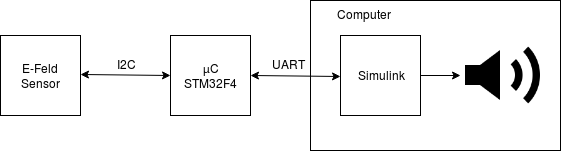
\includegraphics[width=12cm]{MainIdea.png}  
\caption{Simplified project diagram}
\end{figure}

\noindent Because of the lack of previous experience with C, we decided to use Matlab/Simulink and the Waijung blockset for programming the STM32F4Discovery \footnote{A more flexible development option for more experienced developers is the Keil Development Tools program.}. 


\subsection{I2C Communication}

\noindent The Communication between MGC3031 and Host is realized by I2C-Bus. However, the MGC3031 provides two lines that are not implemented in the i2C Bus standard and are needed to use the sensor without restrictions.

\medskip

\noindent The TRANSFER STATUS LINE TS is used by both, the I2C master and slave and is used to check if data is available or ready to be sent. With the TS the usage of the I2C-Bus can be reduced and is advantageous when several slaves are connected to the I2C-Bus. Used as bidirectional line the TS requires an open-drain connection!

\medskip

\noindent In our Solution the TS is not used because we request every 10ms new data from the MGC3130 regardless of new data is available or not.
The second line that is provided by the MGC3031 is the MASTER CLEAR LINE MCLR. It is used by the I2C Master only and is especially needed to update the Firmware of the MGC3031. In our solution the MCLR is not used as we don’t require to update the firmware or to reset the MGC3031.

\medskip

\noindent The MGC3031 has a lot of possibilities to track down movements, a lot of configuration options, provides error detection and it is possible to calibrate the Sensor.
To benefit from all these possibilities the message format and message order are predefined by the MGC3031. Received and send messages have a similar format that consist of Header and Payload.

\medskip

\begin{figure}[h]
\centering
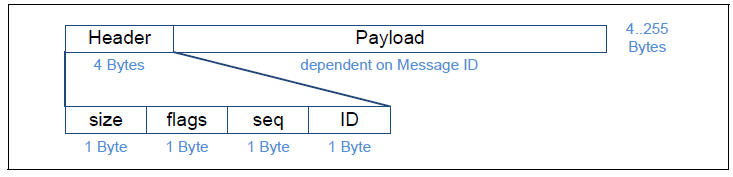
\includegraphics[width=15cm]{Figure1.PNG}
\caption{Datagram structure}
\end{figure}

\medskip

\noindent Header which contains the ID which shows what kind of message is to be received / transmitted and the Payload contains the information to be exchanged. 

\medskip

\noindent Our goal was to configuration the MGC3031 in a way, that it tracks the position of a finger and send only the xyz-coordinate of the tracked position. To accomplish that the RUNTIME\_PARAMETER of the MGC3031 has to be set accordingly.

\medskip

\noindent Each time we send a SET\_RUNTIME\_PARAMETER message the MGC3031 response with a SYSTEM\_STATUS message which includes an ErrorCode that indicates if the setting was successful. Each SYSTEM\_STATUS messages is verified by the program. If one SYSTEM\_STATUS Messages shows an Error the whole initialization is repeated.

\medskip

\noindent After the MGC3031 is initialized the program calls the MGC3031 every 10ms. If there is an object within the range of the sensor the MGC3031 responses with a SENSOR\_DATA\_OUTPUT message which contains the xyz-coordinates. If there is no object within the range of the sensor the MGC3031 responses with a message which only contains zeros. For more information about message format and initialization see appendix.

\newpage

\subsection{Data Processing and Sound output}

\noindent For the instrument playstyle we decided to use the equivalent of a piano key. The area of the sensor was virtually divided into quadrants, each of these quedrants produce a different frequency. For a quadrant to be pressed/active the current XY-position of the finger/object has to be inside the quadrant limits and the Z-Threshold has to be surpassed. The position of the object/finger above the sensor is checked every takt. 

\medskip

\noindent Frenquency values are sent through UART - Protocol to the serial port of a computer. Using the "Tone.slx" Simulink file, the frequency value will be used to create a sinus signal that later is sent to the speakers of the pc. 

\begin{figure}[h]
\centering
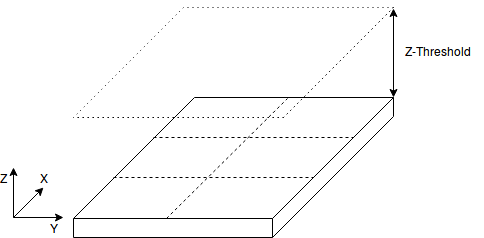
\includegraphics[width=12cm]{SensorKeys.png}
\caption{Key Distribution in sensor}
\end{figure}


\end{document}
